\newpage
\section{Summary}\label{sec:results}
%appliaction of methods
\begin{figure}[ht!]
    \centering
    \begin{subfigure}[b]{\textwidth}
        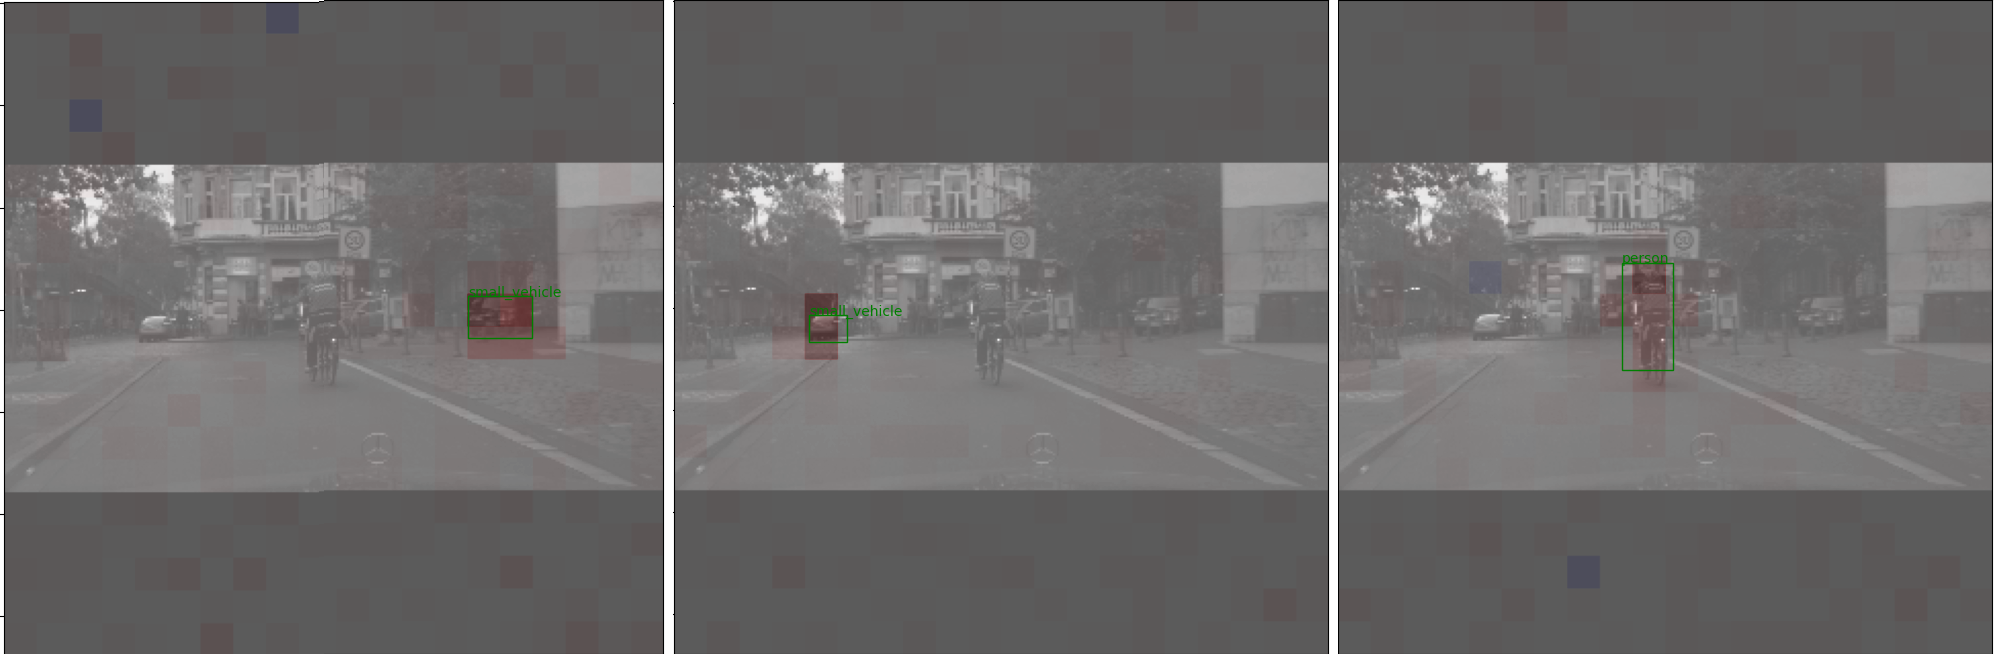
\includegraphics[width=\textwidth]{figures/output}
        \caption{Shapley values of mostly visible objects in the centre of the picture}\label{fig:SHAP_results2}
    \end{subfigure}
    \hfill
    \begin{subfigure}[b]{\textwidth}
        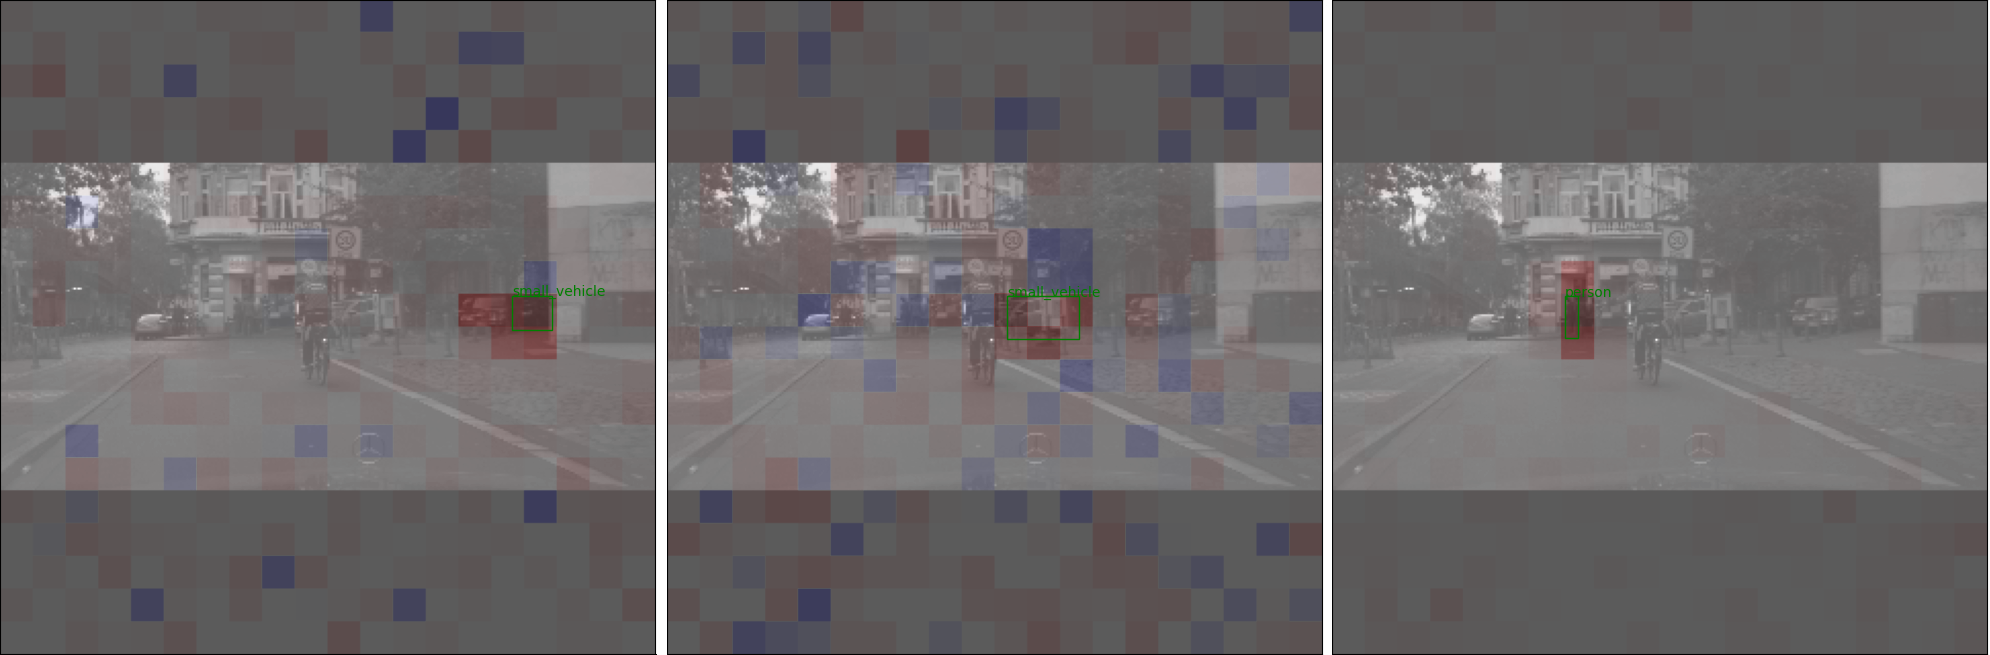
\includegraphics[width=\textwidth]{figures/output2}
        \caption{Shapley values of partially visible objects}\label{fig:SHAP_results20}
    \end{subfigure}
    \hfill
    \begin{subfigure}[b]{\textwidth}
        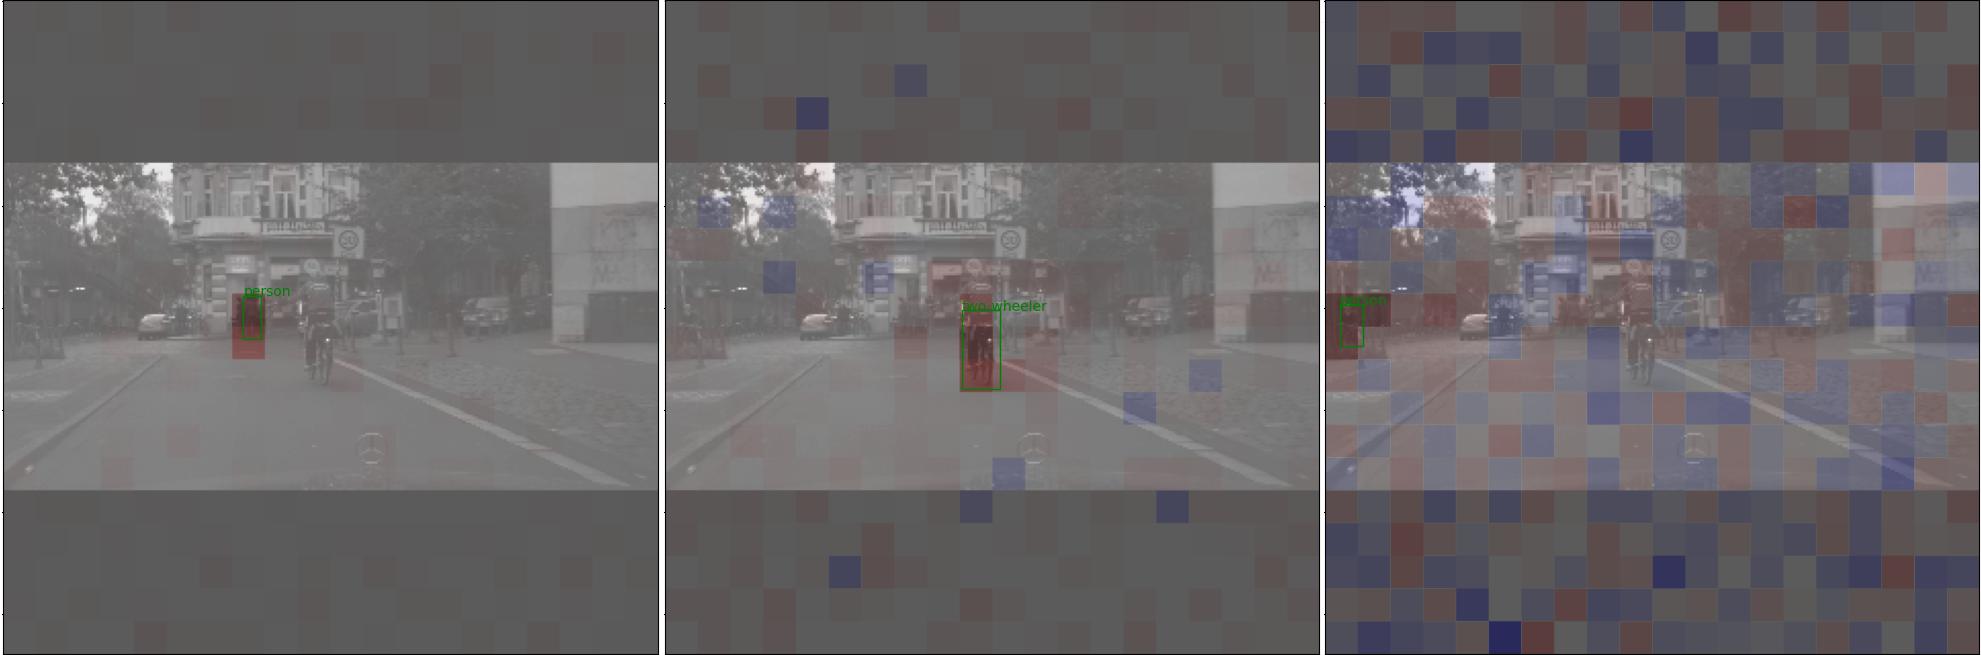
\includegraphics[width=\textwidth]{figures/output2,1}
        \caption{Shapley values for different objects, the object on the side of the image has a low probability of detection, resulting in noise.}\label{fig:SHAP_results21}
    \end{subfigure}
    \hfill
    \begin{subfigure}[b]{\textwidth}
        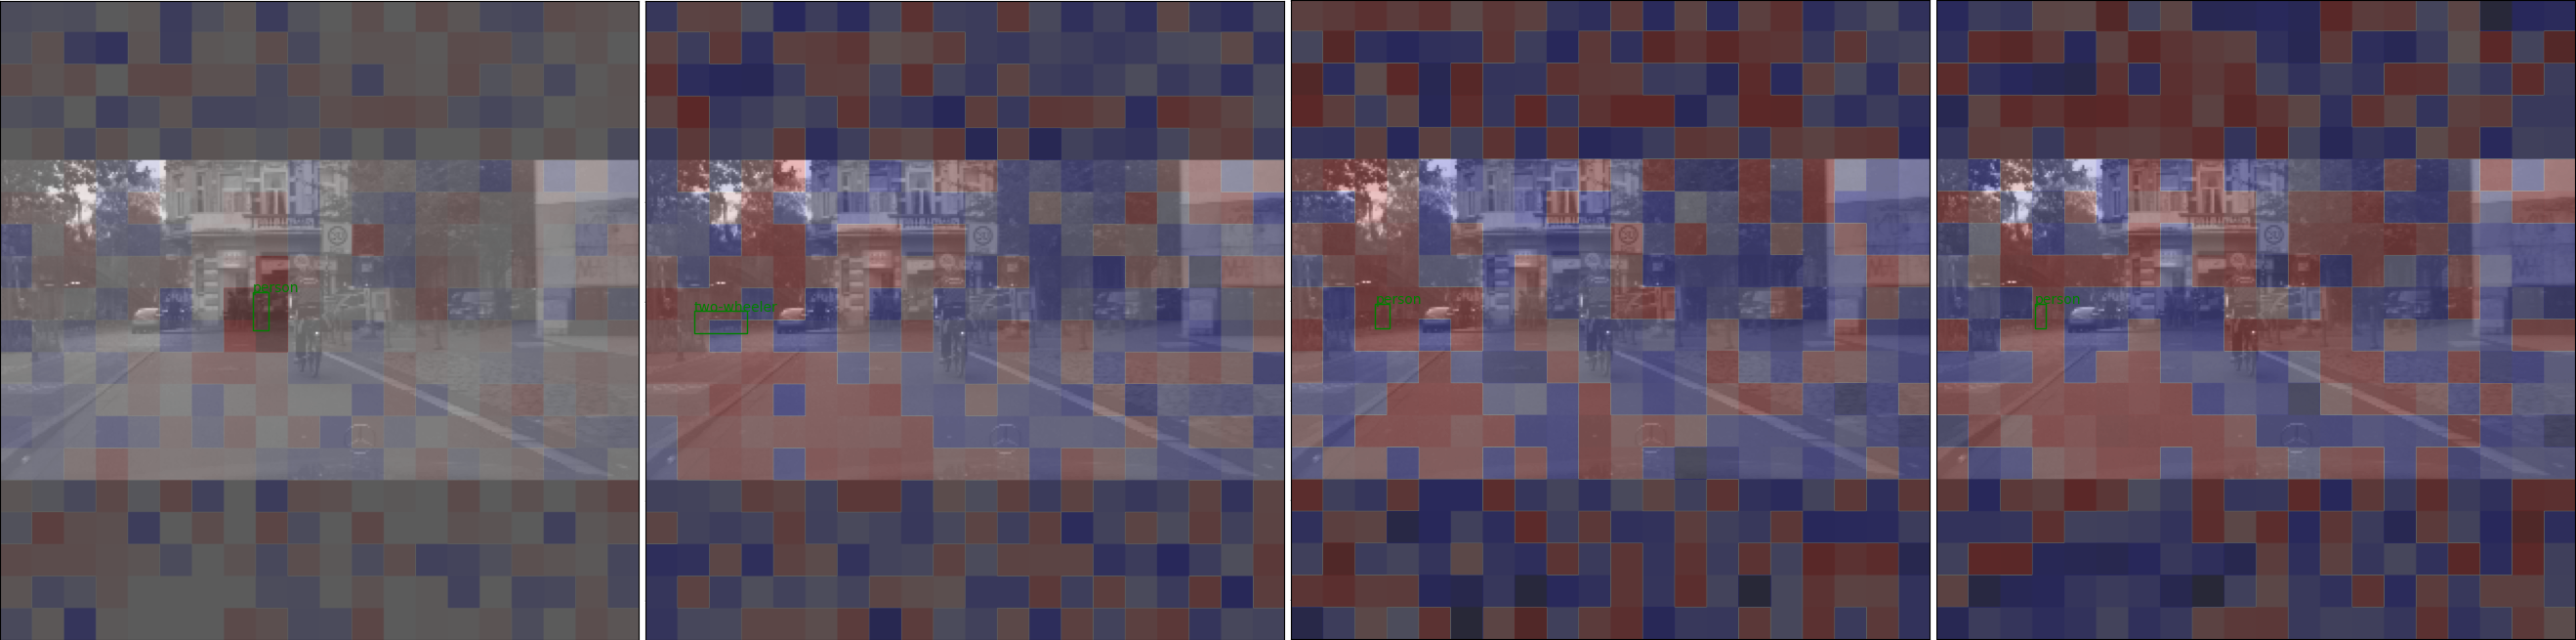
\includegraphics[width=\textwidth]{figures/output2,2}
        \caption{Noisy Shapley values for partially occluded or too small objects }\label{fig:SHAP_results22}
    \end{subfigure}
    \caption{SHAP results for different instances}
    \label{fig:SHAP_results_combined}
\end{figure}
\subsection{Further interpretation results}
\paragraph{Explanation to SHAP (Figure\ref{fig:SHAP_results_combined})}


Top Row (\ref{fig:SHAP_results2}): The overlaid SHAP visualizations suggest which areas were crucial for the model in identifying these objects, which were two cars and the bike-rider.
The highlighted regions are minimal, indicating a high-confidence detection of the object, with the model focusing specifically on the relevant parts of the image.

Top Middle Row (\ref{fig:SHAP_results20}): Here, a broader range of the image is influenced by SHAP values, with more regions showing relevance to the model's predictions.
This suggests that the model is incorporating additional contextual information, such as the surroundings or the road, to reinforce its detection decisions, as well as noise made by the lacking confidence detections of these objects.
The highlighted regions expand around the objects, likely indicating the model's reliance on environmental cues in this analysis level.

Bottom middle Row (\ref{fig:SHAP_results21}): In this row, the SHAP visualization becomes even more widespread, covering a significant portion of the image. This extensive coverage suggests that the model considers a broader context in its decision-making, potentially analysing both relevant and less relevant areas. This could mean that the model is being influenced by more peripheral or background features, reflecting a lower confidence level or a higher sensitivity to context.

Bottom Row(\ref{fig:SHAP_results22}): These pictures are almost entirely made out of noisy explanations of SHAP, caused by the often discussed lack of confidence.



\begin{figure}[h!]
    \centering


    \begin{subfigure}[b]{0.49\textwidth}
        \centering
        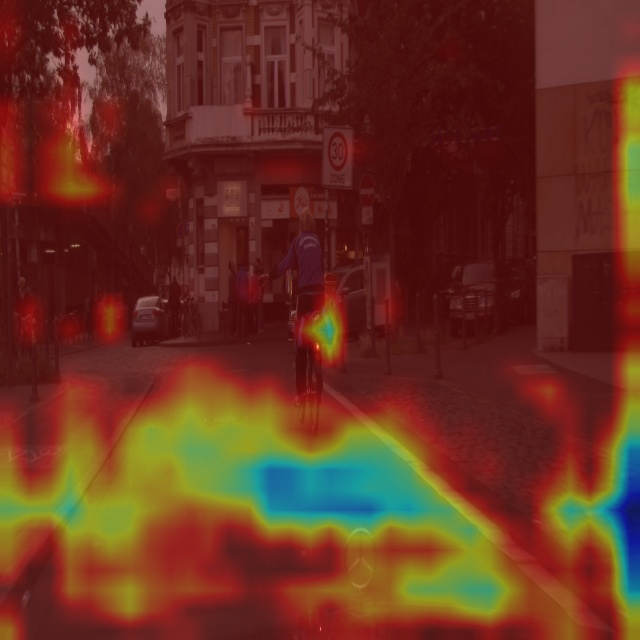
\includegraphics[width=\textwidth]{figures/bonn_000036_000019_leftImg8bit.pnglayer-2/bonn_000036_000019_leftImg8bit.png_object(0)_heatmap}
        \caption{Layer -2}
        \label{fig:b-2}
    \end{subfigure}
    \hfill
    \begin{subfigure}[b]{0.49\textwidth}
        \centering
        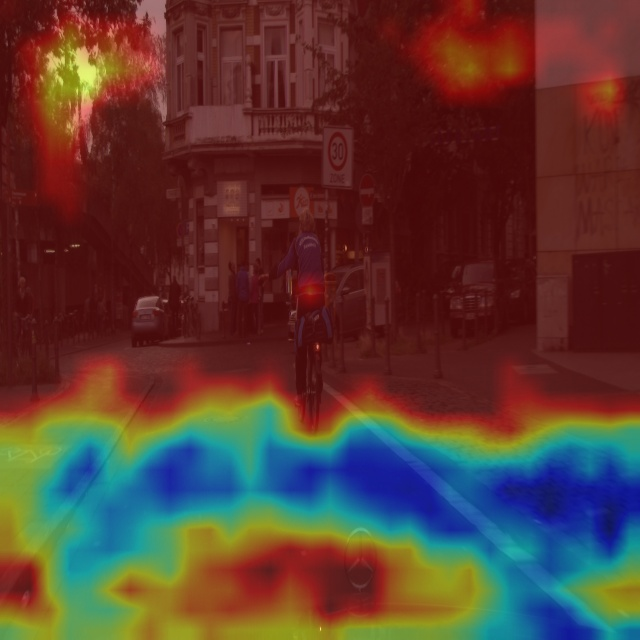
\includegraphics[width=\textwidth]{figures/bonn_000036_000019_leftImg8bit.pnglayer-3/bonn_000036_000019_leftImg8bit.png_object(0)_heatmap}
        \caption{Layer -3}
        \label{fig:b-3}
    \end{subfigure}
    \hfill
    \begin{subfigure}[b]{0.49\textwidth}
        \centering
        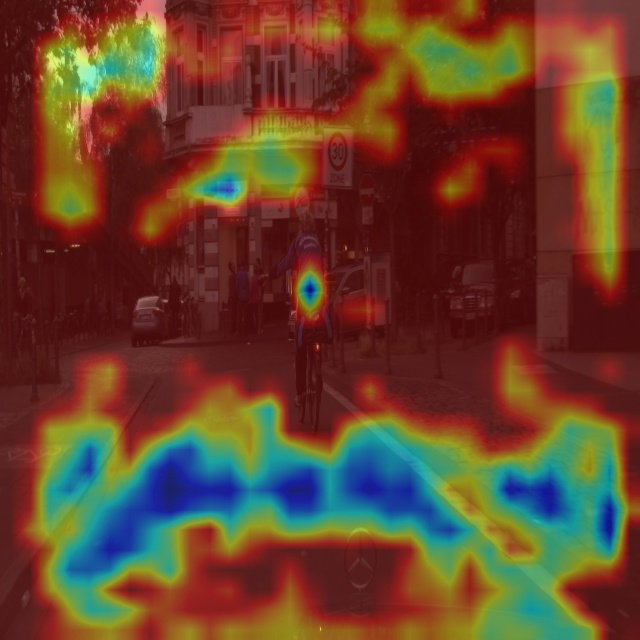
\includegraphics[width=\textwidth]{figures/bonn_000036_000019_leftImg8bit.pnglayer-4/bonn_000036_000019_leftImg8bit.png_object(0)_heatmap}
        \caption{Layer -4}
        \label{fig:b-4}
    \end{subfigure}
    \hfill
    \begin{subfigure}[b]{0.49\textwidth}
        \centering
        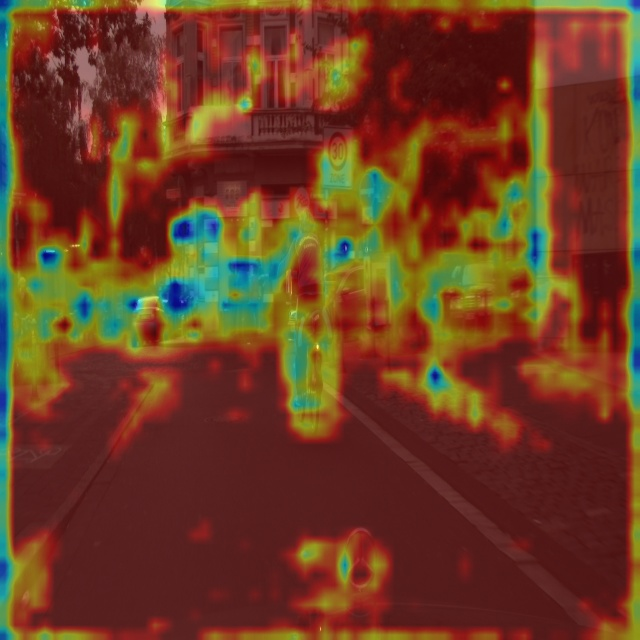
\includegraphics[width=\textwidth]{figures/bonn_000036_000019_leftImg8bit.pnglayer-5/bonn_000036_000019_leftImg8bit.png_object(0)_heatmap}
        \caption{Layer -5}
        \label{fig:b-5}
    \end{subfigure}
    \hfill

    \caption{Activation maps for the Layer -2, -3, -4, -5 for Bonn36}
    \label{fig:Bonn_000036_000019}
\end{figure}
\paragraph{Explanations to EigenCAM results}

\begin{enumerate}
    \item \textit{Layer -2 (\ref{fig:b-2})} : The activation map focuses on the central region, especially around the road and potential objects. The model detects general structures and outlines, emphasizing the primary objects in the scene.
    \item \textit{Layer -3 (\ref{fig:b-3})} : The activation expands slightly, incorporating more background elements, such as buildings and signs. The model begins to consider the broader environment around the primary objects, adding context to the detection.
    \item \textit{Layer -4 (\ref{fig:b-4})} : The activations are more dispersed across the image, covering both foreground and background elements. The model captures finer-grained features, interpreting both the main objects and additional environmental details like signs and building textures.
    \item \textit{Layer -5 (\ref{fig:b-5})} : The activation map is broad and diffuse, with high responsiveness to nearly all elements on the image, including roads, buildings, trees, and signs. The model at this stage captures complex, scene-wide patterns, and high-level feature representations.
\end{enumerate}


\begin{figure}
    \centering
    \begin{subfigure}[b]{0.49\textwidth}
        \centering
        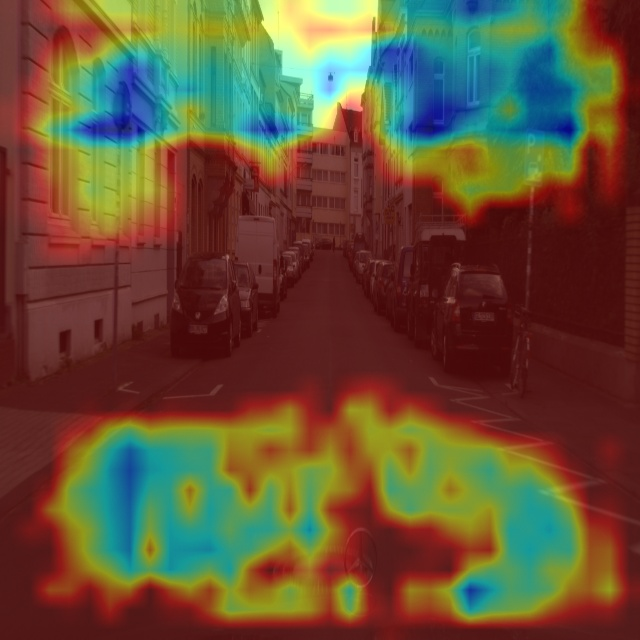
\includegraphics[width=\textwidth]{figures/bonn_000037_000019_leftImg8bit.pnglayer-2/bonn_000037_000019_leftImg8bit.png_object(0)_heatmap}
        \caption{Layer -2}
        \label{fig:c-2}
    \end{subfigure}
    \hfill
    \begin{subfigure}[b]{0.49\textwidth}
        \centering
        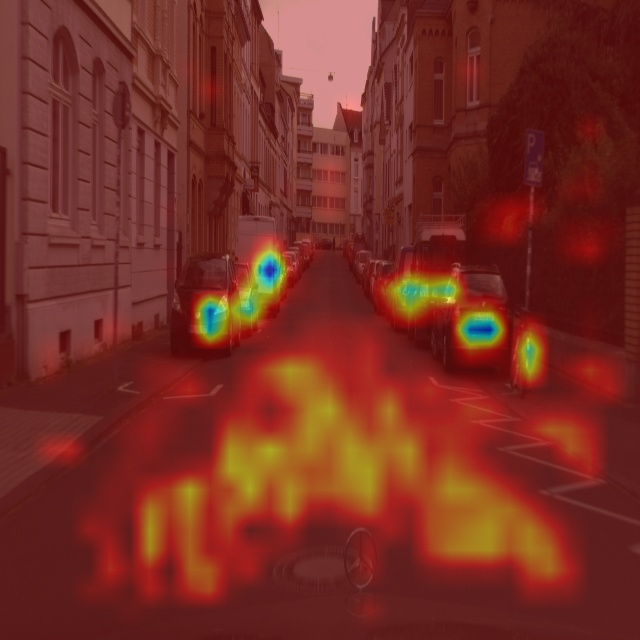
\includegraphics[width=\textwidth]{figures/bonn_000037_000019_leftImg8bit.pnglayer-3/bonn_000037_000019_leftImg8bit.png_object(0)_heatmap}
        \caption{Layer -3}
        \label{fig:c-3}
    \end{subfigure}
    \hfill
    \begin{subfigure}[b]{0.49\textwidth}
        \centering
        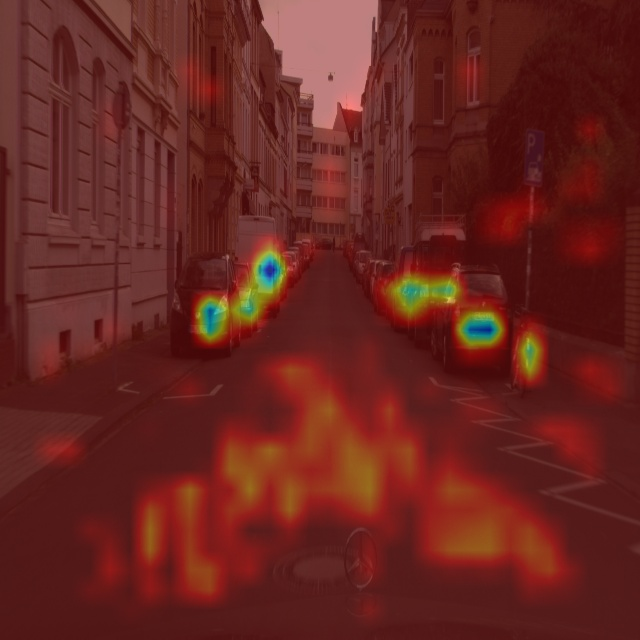
\includegraphics[width=\textwidth]{figures/bonn_000037_000019_leftImg8bit.pnglayer-4/bonn_000037_000019_leftImg8bit.png_object(0)_heatmap}
        \caption{Layer -4}
        \label{fig:c-4}
    \end{subfigure}
    \hfill
    \begin{subfigure}[b]{0.49\textwidth}
        \centering
        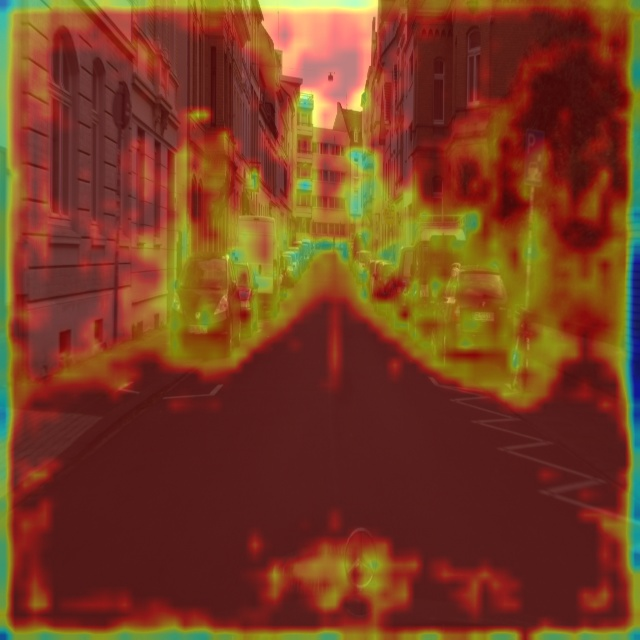
\includegraphics[width=\textwidth]{figures/bonn_000037_000019_leftImg8bit.pnglayer-5/bonn_000037_000019_leftImg8bit.png_object(0)_heatmap}
        \caption{Layer -5}
        \label{fig:c-5}
    \end{subfigure}
    \hfill
    \begin{subfigure}[b]{0.49\textwidth}
        \centering
        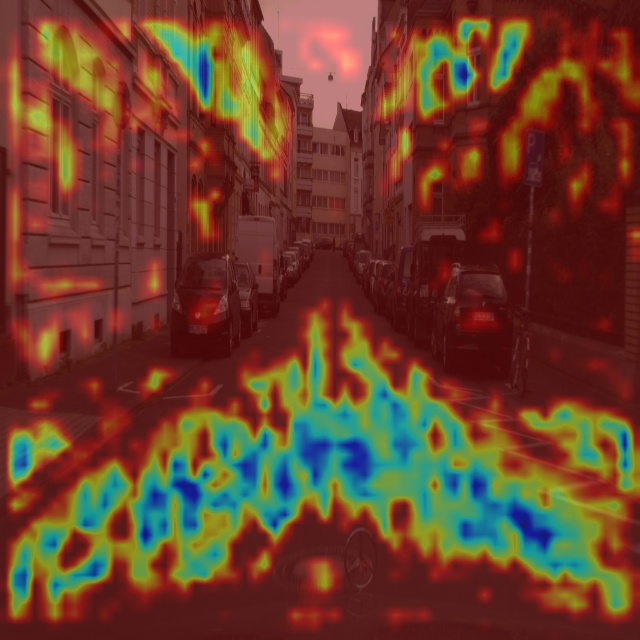
\includegraphics[width=\textwidth]{figures/bonn_000037_000019_leftImg8bit.pnglayer-6/bonn_000037_000019_leftImg8bit.png_object(0)_heatmap}
        \caption{Layer -6}
        \label{fig:c-6}
    \end{subfigure}
    \hfill
    \caption{Activation maps for the Layer -2, -3, -4, -5 for Bonn37}
    \label{fig:Bonn-000037-000019}
\end{figure}

Explanations for Figure~\ref{fig:Bonn-000037-000019}:
\begin{enumerate}
    \item \textit{Layer -2 (\ref{fig:c-2})}: The activation map shows focus on both the top and bottom regions of the image, capturing general structural elements, such as the sky at the top and the street at the bottom. This layer mainly highlights broad spatial features without much fine detail.
    \item \textit{Layer -3 (\ref{fig:c-3})}: Activations become more specific with a focus on distinct points along the street. This suggests that the model is beginning to identify specific objects or areas of interest along the roadway, possibly focusing on features relevant to the street layout or potential objects in the environment.
    \item \textit{Layer -4 (\ref{fig:c-4})}: The model's focus widens, capturing both sides of the street more prominently, with activations spreading across buildings and other elements lining the road. This indicates a balance between object-specific and context-specific features, as the model integrates more scene context.
    \item \textit{Layer -5 (\ref{fig:c-5})}: The activation is more expansive, covering almost the entire image, particularly emphasizing areas surrounding the street. This layer appears to interpret larger, scene-wide patterns, possibly identifying the overall structure of the street and surrounding buildings.
    \item \textit{Layer -6 (\ref{fig:c-6})}:  Activations spread densely throughout the image, with a particular focus on the length of the street and the buildings that line it. This deep layer captures high-level abstractions, incorporating nearly the entire scene, reflecting the model's comprehensive understanding of the spatial layout and contextual details.

\end{enumerate}

\subsection{Takeaways}\label{subsec:takeaways-and-suggestions-for-future-development}


Notable advancements have been made in the interpretation and explanation of the behaviours exhibited by computer vision models, particularly through the application of SHAP and EigenCAM.
These tools have facilitated a more profound understanding of the decision-making processes of intricate models, thereby offering a more transparent view of the manner in which these models prioritise and process visual information in different contexts.
In particular, SHAP facilitated interpretability by decomposing model predictions into feature contributions.
EigenCAM, on the other hand, used activation-based heat maps to visualise the model's spatial awareness.

While the results of LIME were less conclusive in this context, possibly due to challenges in its level of complexity compared to the model's architecture, the combined use of SHAP and EigenCAM successfully illustrated the potential for effective and detailed visualisations of model interpretations.
By observing SHAP and EigenCAM outputs on the same image, we were able to achieve a more comprehensive view of model processing, providing a multi-faceted perspective on how the model detects and evaluates objects.
This approach represents a step towards a comprehensive, global understanding of model behaviour through the integration of individual, local interpretations, where the strengths of each method complement the limitations of the other.

The robustness and accuracy of Yolov8 on the Cityscapes dataset further validated its ability to handle complex real-world scenes, particularly urban environments where object detection tasks can be challenging due to varying object scales, densities, and positions. Yolov8 demonstrated superior performance in accurately identifying a wide range of objects within the dataset - such as pedestrians and different vehicles - across different spatial arrangements, reflecting its resilience and adaptability to real-world applications.
This consistency across different scenarios within the Cityscapes dataset underscores Yolov8's potential for use in applications that require high precision, such as autonomous driving and urban planning.

The successful application of Yolov8 in combination with interpretability methods such as SHAP and EigenCAM highlights a promising path for future computer vision models.
This combined approach suggests that powerful models can also be interpretable, promoting transparency without compromising performance.
This integration of interpretability tools with powerful models such as Yolov8 offers exciting possibilities for future work, such as real-time applications where both accuracy and transparency are paramount, ultimately contributing to the development of trustworthy, interpretable, and powerful computer vision systems.

\subsection{Directions for further development}\label{subsec:dircetions-for-further-development}

Although this project has made considerable progress in clarifying the functioning of models in the domain of computer vision, there are still numerous avenues for further investigation and development.

Firstly, enhancing the interpretability of underperforming methods, such as LIME, could improve the consistency and reliability of model explanations across various instances.
Further investigation of parameter tuning or alternative implementations of LIME may facilitate the development of more robust explanations.

Furthermore, it would be beneficial to implement other, less well-known methods, or to revisit the approaches discussed in previous subsections (\ref{sec:model-interpretation}), such as adversarial-based interpretation methods, for example Anchor \cite{LIANG2021168}.
Additionally, EigenGradCAM could be utilized or another model-specific method could be employed to gain a deeper comprehension of the model's internal operations by elucidating the training process.

Furthermore, the integration of interpretability techniques, such as SHAP and EigenCAM, into real-time applications represents a promising avenue for future research.
Further work could concentrate on optimising these methods to operate effectively in conjunction with the model.

An expansion of the interpretability framework to include other datasets beyond Cityscapes would serve to further test the model's adaptability and the scalability of the interpretability methods across different environments. In addition, the incorporation of a more extensive range of data could facilitate a more comprehensive understanding of the generalizability and limitations of the model.

Finally, efforts could be directed towards the development of unified visualization tools that allow for dynamic, interactive exploration of combined interpretations from multiple methods.
Such tools would enable researchers and practitioners to better analyse, understand and refine model behaviour across complex tasks, ultimately fostering greater trust and transparency in computer vision systems.


